\section{Game Theory}
\label{sec:game-theory}

\vspace{1cm}

\begin{figure}[h]
  \label{fig:paradise}
  \centering
  \fcolorbox{black}{white}{
    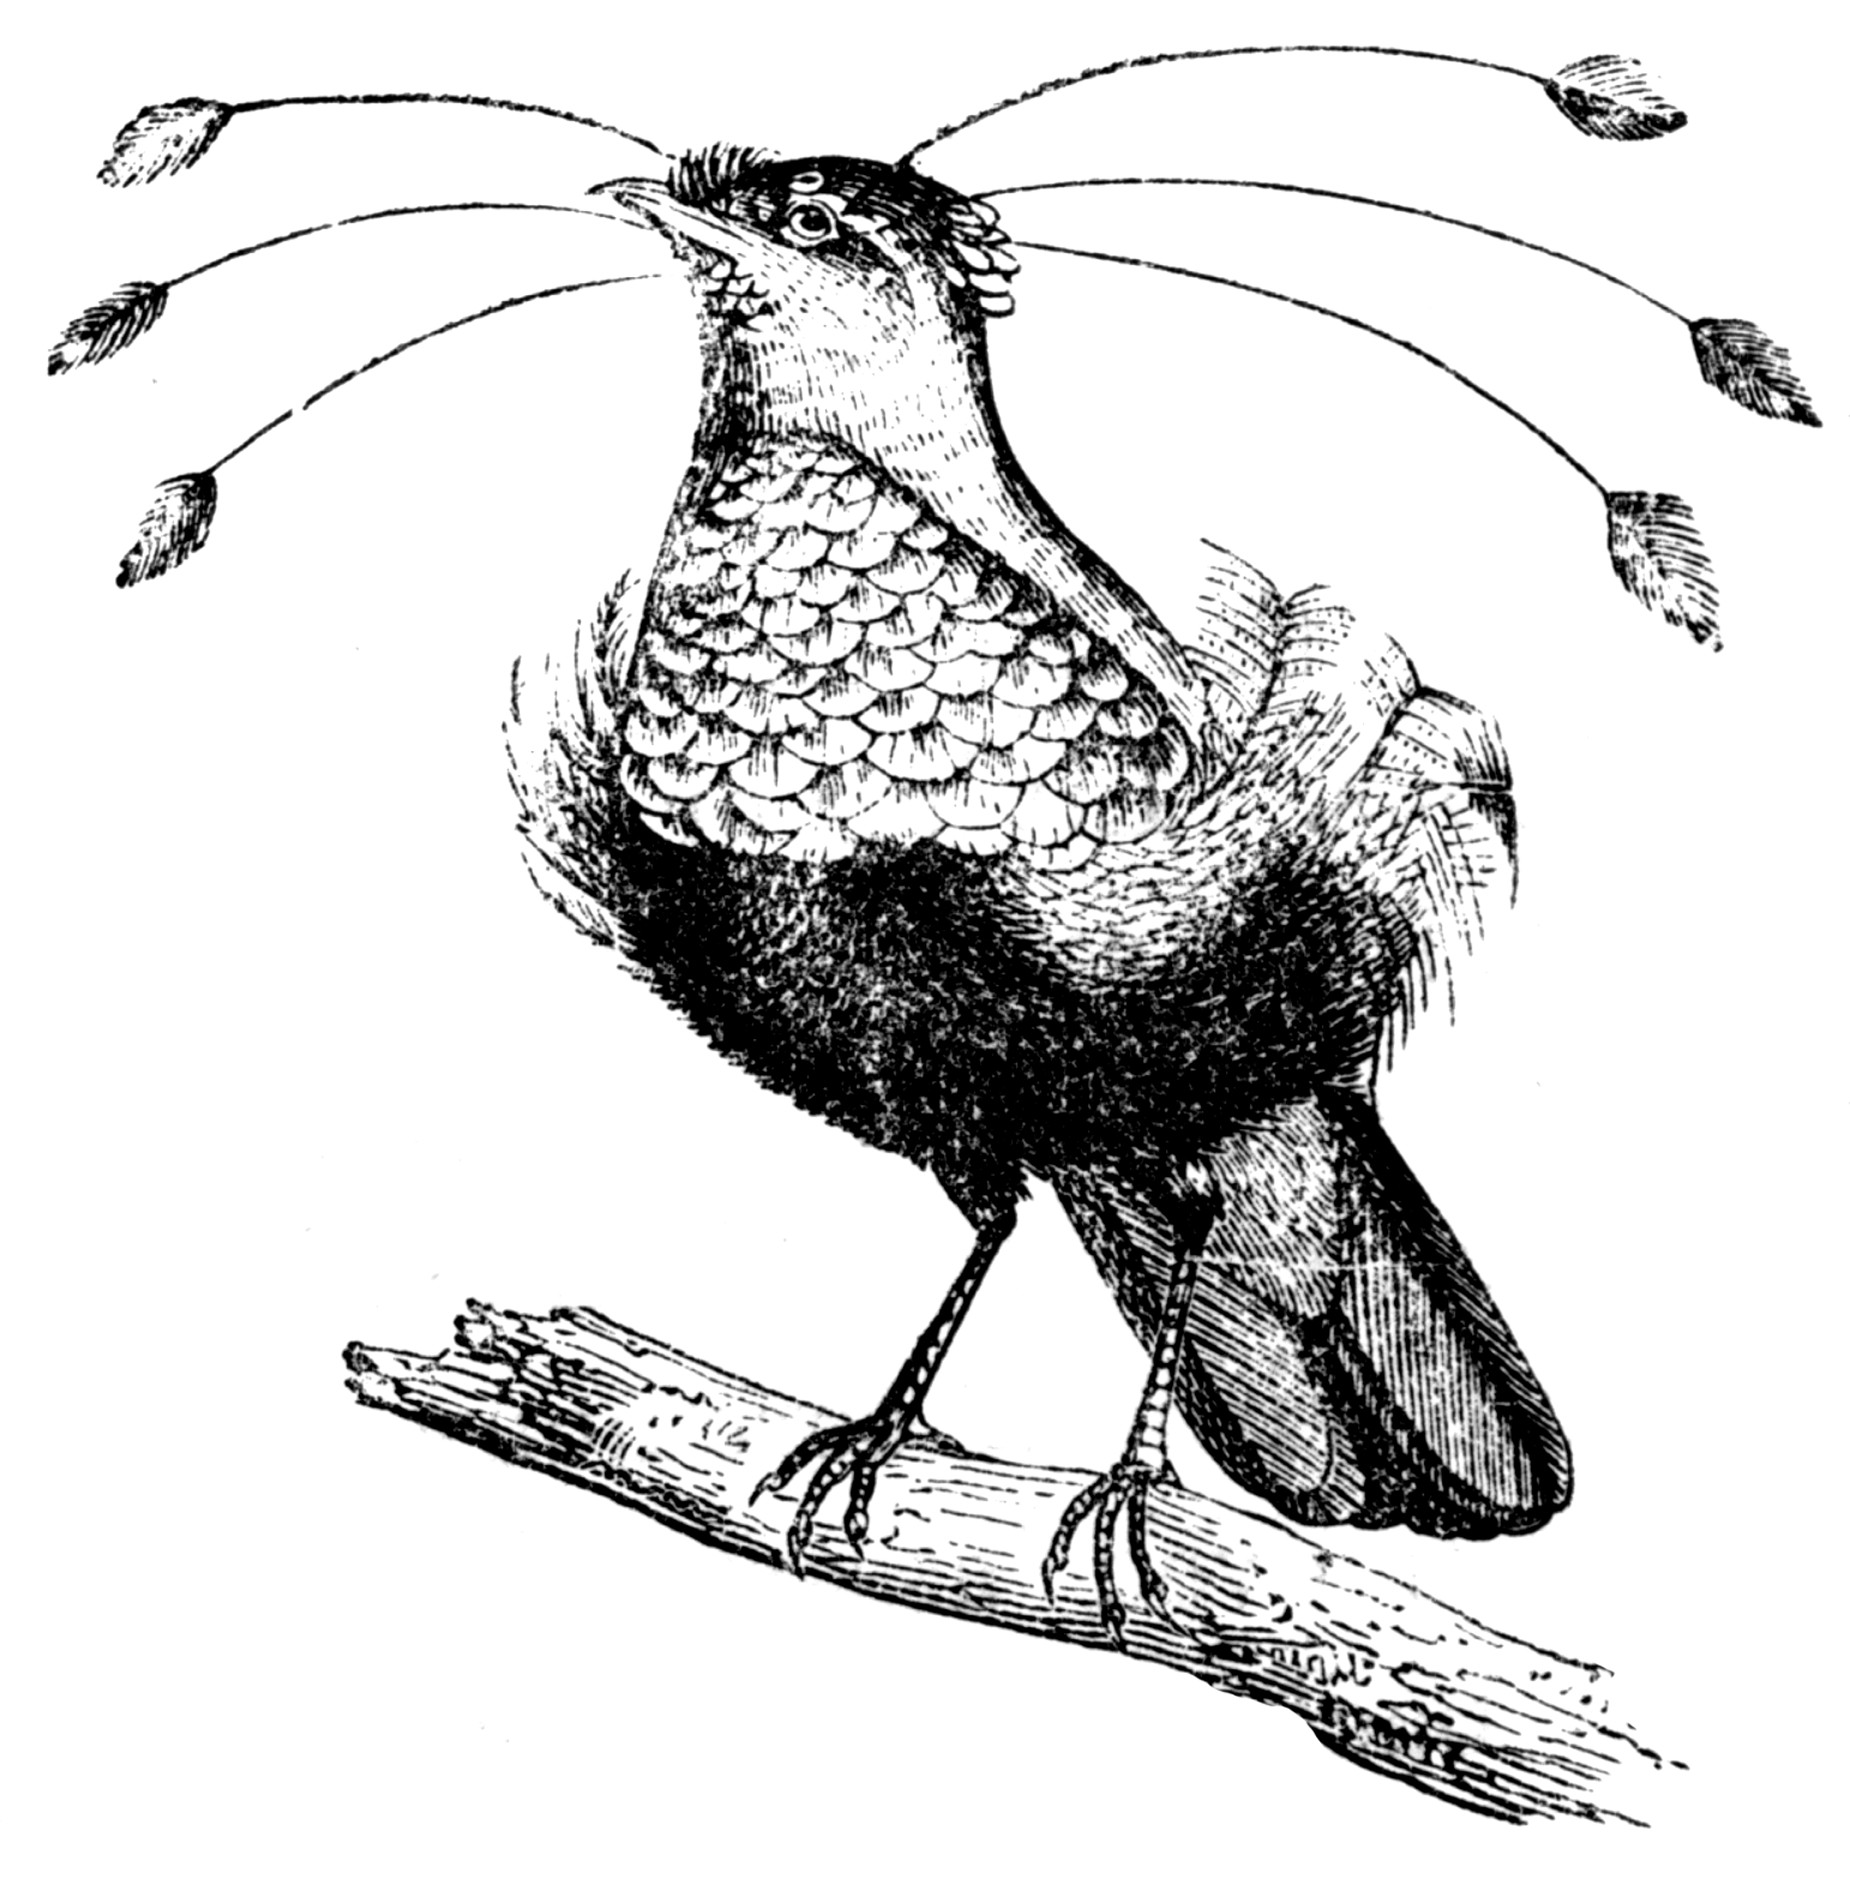
\includegraphics[width=0.3\textwidth]{paradise}
  }
  \caption{Louis Figuier, ``Reptiles and Birds'', 1869.}
\end{figure}

\vspace{1cm}

\noindent The original theoretical formulation of the GAN algorithm,
as in~\cite{ref:goodfellow-original}, is through \textit{game theory},
which is the study of conflict and cooperation between rational
decision makers through the use of mathematical and statistical
modeling~\cite{ref:myerson}.  Throughout this paper we only consider
two-player games, and we will use $D$ to represent the player, and $G$
to represent her opponent. We use the symbol $V_i$ to represent the
value function of player $i$ for $i \in \{D, G\}$.

\begin{definition}
  \label{def:value-function}
  A \textnormal{\sffamily value function} $V_i$ is the reward (or loss
  if it is negative) for player $i$ in a game as a function of that
  player's action(s).
\end{definition}

\begin{remark} Sometimes the loss is simply the difference between the
  target value $y$ and the estimate $\hat{y}$. In the case of GANs,
  the value function is more complex, and is essentially a measure on
  uncertainty.
\end{remark}

There are actually two value functions (see Section
\ref{sec:two-value}) used in \cite{ref:goodfellow-original}, the first
allows the GAN algorithm to be interpreted as a \textit{zero-sum
  game}, while the second value function does not
\cite{ref:gidel-variational-2018}.

\begin{definition}
  \label{def:zero-sum-game} A \textnormal{\sffamily zero-sum game} is
  any game where the loss of one player is the gain of the other. In a
  zero-sum game, the players' rewards sum to zero, i.e.
  $V_D + V_G = 0$.
\end{definition}

\begin{remark} For this section we will stick with the the first value
  function, therefore we will consider the GAN algorithm to be a
  zero-sum game between the generator and the discriminator, see
  (\ref{def:generator}) and (\ref{def:discriminator}) for the relevant
  definitions.
\end{remark}

What is the optimal strategy in a zero-sum-game? At any given turn,
what action should a player take to maximize his or her chances of
winning or at least minimize the expected loss? The \textit{minimax
  decision rule} is a strategy to get the best outcome given that you
know your opponent is trying to minimize your reward.

\begin{definition}
  \label{def:minimax}
  \label{def:minimax-value} In a two-player game, with players $D$ and
  $G$, a \textnormal{\sffamily minimax decision rule} for $D$ is a
  strategy that maximizes $D's$ expected reward, after $G$ has
  minimized the maximum reward attainable by $D$ that is. The
  \textnormal{\sffamily minimax value} $\overline{V_D}$ for $D$, is
  the largest reward $D$ can win after $G$ makes his move to minimize
  $D$'s reward, in symbols we write
  \begin{align} \overline{V_D} = \min_{G} \max_{D} V_D(D, {G}).
  \end{align}
\end{definition}

In a game between $D$ and $G$, if $G$ moves first to minimize the
reward $D$ can attain on her move, the minimax rule for $D$ will allow
$D$ to attain the maximum of the reduced reward.

\subsection{Nash Equilibrium and the Prisoner's Dilemma}
\label{sec:nash-dilemma}

The GAN algorithm searches for a \textit{Nash equilibrium} in the
space of parameters for the discriminator and the generator, as covered
in \cite{ref:goodfellow-2016} and \cite{ref:goodfellow-2017}.

\begin{definition}
  A \textnormal{\sffamily Nash equilibrium} in an $n$-player game is a
  set of strategies, one for each player, with the property that no
  player can benefit from unilaterally changing their strategy.

  Let $S_i$ denote the set of strategies for player $i$. Let
  $S = S_1 \times S_2 \times \cdots \times S_n$ denote the set of
  strategy profiles.  Each strategy profile $s \in S$ is a combination
  of strategies, one for each player, which dictates what each player
  will do on their next turn.  Let $f_i(s)$ be the payoff to player
  $i$ of strategy profile $s$.

  A Nash equilibrium is a strategy profile
  $s^* = (s_1, s_2, \dots, s_n)$ such that
  \begin{align}
  f_i(s^*) \geq f_i((s_1, s_2, \dots, s_{-i}, \dots, s_n))
  \end{align}
  for all $i$ and $s_{-i}$ denotes any strategy of player $i$ other
  than $s_i$ from $s^*$.
\end{definition}

\begin{remark}
  Each player's strategy is an optimal response based on the
  anticipated behavior of the other player(s) in the game.  A minimax
  solution to a zero-sum game is the same as a Nash Equilibrium. The
  Nash equilibrium is not necessarily globally optimal and a game may
  have more than one Nash equilibrium.
\end{remark}

% \begin{remark}
%   Nash's existence theorem states that for $S_i$ for all $i$ and for
%   finite $n$, at least one Nash equilibrium exists.  For more
%   information, see \cite{ref:nash-1950} and \cite{ref:nash-1951}.
% \end{remark}

We look to the \textit{Prisoner's Dilemma} for an illustrative example
of a Nash equilibrium. The Prisoner's Dilemma was originally
formulated in a paper by Merrill Flood and Melvin Dresher in the
1950s, and Albert W. Tucker reformulated the game in terms of prison
sentences and gave it the name \textit{Prisoner's Dilemma}
\cite{ref:poundstone}. The point of the Prisoner's Dilemma is to show
that the globally optimal state may not be realistically attainable in
a non-cooperative game. Each player is trying to minimize their
expected jail-time, and they are assuming the other player is doing
the same, and given that, they will not achieve the global minimum.

\subsubsection{Prisoner's Dilemma}
\label{sec:prisoners-dilemma}

This game has two players, $D$ and $G$, who are held separately in
police custody with no means of communication. The players have each
been arrested for some small crime which the prosecution has enough
evidence to convict them of. However, the prosecution suspects one of
$D$ or $G$ of having committed a more serious crime in the
not-so-distant past. The problem is they lack sufficient evidence to
convict either $D$ or $G$ of the more serious crime. So the
prosecutors cut each player a deal. The deal is

\begin{enumerate}
\item if $D$ defects and accuses $G$ of having committed the more
  serious crime (and $G$ denies involvement) $D$ gets 1 year (as a
  reward for co-operation) while $G$ gets 5 years of jail-time (and
  vice-versa);
\item if both $D$ and $G$ deny committing the larger crime, then they
  both get 2 years, since the prosecution does have enough evidence to
  convict them of the less serious crime;
\item if both $D$ and $G$ accuse each other of committing the larger
  crime, then they both get 3 years. Remember, they can not
  communicate with each other.
\end{enumerate}

\begin{figure}[h] \centering \bgroup \def\arraystretch{1.4}
  \begin{tabular}[c]{|c|c|c|}
    \hline
    \diagbox{$D$}{$G$} & Deny & Defect \\
    \hline
    Deny & (2, 2) & (5, 1) \\
    \hline Defect & (1, 5) & (3, 3) \\
    \hline
  \end{tabular} \egroup
  \caption{Prisoner's Dilemma Payoff Matrix}
  \label{fig:prisoners-matrix}
\end{figure}

Figure~\ref{fig:prisoners-matrix} has the game's payoff matrix, scores
are for ($D$, $G$), i.e. $D$ controls the rows and $G$ controls the
columns. It's obvious that (Deny, Deny) is the global optimum, but it
turns out that it's an unstable state. The state (Defect, Defect) is
the Nash equilibrium, we will go over all four states and show why
this is true.

\begin{enumerate}
\item \textit{(Deny, Defect).} If $D$ is allowed to change her stance,
  knowing that $G$ is going to defect, she will end up in a better
  situation, which means there is incentive for $D$ to change her
  strategy, given that $G$ will not change his. Therefore, this is not
  a Nash equilibrium, and vice-versa for (Defect, Deny) by symmetry.
\item \textit{(Deny, Deny).} If $D$ and $G$ both deny involvement, and
  if $D$ knows that $G$ is not going to change his stance, $D$ does
  gain from changing her strategy to defecting, since that will change
  the situation to (Defect, Deny), where $D$ does 1 year and $G$ does
  5.
\item \textit{(Defect, Defect).} If they both defect, neither $D$ nor
  $G$ will gain anything by changing their strategy, for if $D$
  changed to denying involvement, $D$ would serve 5 years, and the same
  holds true for $G$.
\end{enumerate}

Thus (Defect, Defect) is the Nash equilibrium for this game. It's a
stable game state, i.e. there is no incentive for either player to
change strategy (unless the other does as well). As $D$ sits in the
holding cell, she is thinking that $G$ is going to either defect or
deny involvement. If $D$ wants to minimize the maximum amount of
jail-time she could possibly do, she will want to defect, since that
will eliminate the worst case scenario of having to do 5 years. When
she defects, the worst that can happen to her is 2 years.

Since in this situation, the minimax does not achieve the global
minimum, what can we say about the minimax strategy and the GAN
algorithm?

\subsection{Derivation of the Value Function}
\label{sec:derivation}

Now that we have introduced the relevant concepts from game theory we
can introduce the algorithm and its constituent neural networks. Let
$(\target, \pt)$ be a probability space where $\target$ is any finite
space. Let $\pt$ be the probability distribution over this space. For
instance $\target$ may be the idealized space of all 8-bit RGB images
of length $H$ and width $W$, i.e.
$\target = [0, 255]^{3 \times H \times W}$, and $\pt$ is the
probability distribution over this space which assigns mass to regions
of $\target$ which correspond to RGB values that look like meaningful
images, e.g.\ images of human faces. Each point in this space
represents an image, and most points in this space will look like
meaningless noise. \footnote{Meaningless to a human.}

The goal of the GAN algorithm is to train a generator $\G$,
parameterized by $\phi \in \Phi \subset \R^n$, to map random samples
$z$ drawn from $(\prior, p_{\prior})$, where $\prior \subset \R^n$
such that $\G(z)$ is located in $\target$ in a region where $\pt$
assigns a relatively large amount of mass. In practice
$\prior \not = \target$ and $n$ is usually smaller than $|\target|$
\cite{ref:arjovsky-2017}.

\begin{figure}[H] \centering
  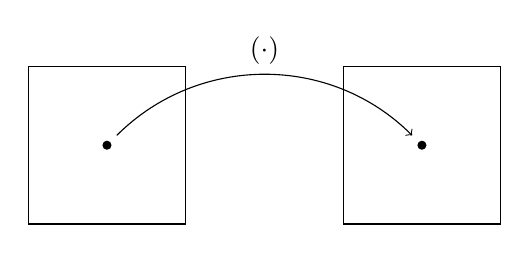
\begin{tikzpicture} \node (G) at (3, 2.2) {$\G(\cdot)$}; \draw (0,
    0) rectangle +(2, 2); \node at (0.2, 1.8) {$\prior$}; \filldraw
    (1, 1) circle (0.05cm); \node (Z) at (1, 1) {}; \draw (4, 0)
    rectangle +(2, 2); \filldraw (5, 1) circle (0.05cm); \node (O) at
    (5, 1) {}; \node at (5.8, 1.8) {$\target$}; \draw[->] (Z) to
    [out=45,in=135] (O);
  \end{tikzpicture}
  \caption{$\G$ maps $z$ to $\G(z) \in \target$}
  \label{fig:g-maps}
\end{figure}

The reason we use a generative model is to obtain samples from
$\target$ characterized by a specific distribution of values. For
instance if $\target$ is the space of all RGB images and we desire
images of human faces, then we want $\G$ to map samples from $\&Z$ to
the region of $\target$ with RGB values within a very narrow range.

In the beginning $\G$ maps $z \in \&Z$ to $\target$ haphazardly and
it is from $\D$ that $\G$ obtains gradients to learn from. We optimize
the discriminator $\D$ until it classifies samples sufficiently well,
i.e. $\D$ must learn to assign the correct probability that the sample
came from the target distribution. Thus $\D$ and $\G$ both learn
$\pt$, but from different perspectives.

Let $\D$ be a discriminator and $\G$ be a generator. Let $\V$ be the
value function, which is a function of the \textit{actions} (which are
parameterized by $\phi$ and $\theta$) taken by $\D$ and $\G$, given by
\begin{align}
  \label{eq:the-original-objective-function}
  \V = \mathbb{E}_{x \sim \pt}[{\log D_\theta(x})] +
  \mathbb{E}_{z \sim \pz}[\log{(1 - D_\theta(G_\phi(z)))}].
\end{align}

The value function used by the GAN algorithm is related to the value
function used by the \textit{noise-contrastive estimator}, see
\cite{ref:gutmann-2010} for more details. In the game between $\G$ and
$\D$, each will want to maximize the minimum reward it can earn and
equivalently, minimize the maximum loss. In general, a player can
minimize the maximum loss by playing its minimax decision rule (see
Definition \ref{def:minimax}).

\subsubsection{Derivation of the Value Function from the Perspective of $\D$}
\label{sec:derivation-d}

We begin the derivation of $\V$ from the perspective of $\D$. We want
$\D(x)$ to assign mass to $x \in \target$ that are close to the mass
assigned by $\pt$. We can do this by finding $\theta \in \Theta$ which
maximize the likelihood function
\begin{align}
  \label{eq:d-1}
  L_{D}^{(1)}(\theta) = \prod_{i=1}^n \D(x_i), \quad x_i \sim \pt.
\end{align}
Since this maximization is done numerically, we maximize the logarithm
of the above equation,
\begin{align}
  \label{eq:d-l1}
  \ell_{D}^{(1)}(\theta) = \log \prod_{i=1}^n \D(x_i) = \sum_{i=1}^n \log \D (x_i).
\end{align}
One benefit of using $\log$ is it is monotone increasing (any argument
that maximizes (\ref{eq:d-l1}) will also maximize (\ref{eq:d-1})) and
the curvature of $\log$ may make optimization more efficient by
providing steeper gradients.

At the same time, since we also want the discriminator $\D$ to
distinguish generated samples from real samples, we want $\D$ to
assign low probability (preferably zero) to any generated data point
$\G(z) = \tilde{x}$.  Therefore, for some fixed $\G$, $\theta$
must also minimize the following likelihood function,
\begin{align}
  ^*L_{D}^{(2)}(\theta) = \prod_{i=1}^n D_\theta(\Gzi), \quad z_i \sim \pz,
\end{align}
and as before, minimization of $^*L_{D}^{(2)}(\theta)$ can be done via
minimization of its logarithm,
\begin{align}
  \label{eq:d-l2} ^*\ell_{D}^{(2)}(\theta) = \log \prod_{i=1}^n D_\theta(\Gzi) = \sum_{i=1}^n \log \D (\Gzi).
\end{align}
Alternatively, since we are already maximizing (\ref{eq:d-l1}), we can
turn (\ref{eq:d-l2}) into a function to be maximized. Specifically, we
ask $\D$ to maximize
\begin{align}
  \ell_{D}^{(2)}(\theta) = \sum_{i=1}^n \log{(1 - D_\theta(G_\phi(z_i)))},
\end{align}
since minimizing $\D(\G(z))$ is the same as maximizing
$1 - \D(\G(z))$. When we combine $\ell_{D}^{(1)}(\theta)$ and
$\ell_{D}^{(2)}(\theta)$ we arrive at the following objective function
for $\D$ to maximize,
\begin{align}
  \sum_{i=1}^n \left( \log D_\theta(x_i) + \log{(1 - \D(\G(z_i)))} \right).
\end{align}
This is equivalent to maximizing the mean, which, by the law of large
numbers, converges to
\begin{align}
  \label{eq:objective-for-d}
  \mathbb{E}_{x \sim \pt}[{\log \D(x})] + \mathbb{E}_{z \sim \pz}[\log{(1 - \D(\G(z)))}]
\end{align}
for $n$ sufficiently large. Thus, we can say the objective of the GAN
algorithm from the perspective of the discriminator is to find a set
of parameters $\theta$ which maximize (\ref{eq:objective-for-d}).

\subsubsection{Derivation of the Value Function from the Perspective of $\G$}
\label{sec:derivation-g}

From the perspective of the generator, we search for $\phi$ that
maximizes the likelihood (as a defined by a fixed $\D$) that a
generated sample comes from the target distribution $\pt$, i.e.\ we
want $\G$ to maximize
\begin{align}
  ^*\ell_G(\phi) = \log\prod_{i=1}^n\D(\G(z_i)) = \sum_{i=1}^n\log{\D(\G(z_i))}, \quad z_i \sim \pz.
\end{align}
Alternatively, we can minimize
\begin{align}
  \ell_G(\phi) = \sum_{i=1}^n\log{(1 - \D(\G(z_i)))},
\end{align}
which is equivalent to minimizing $\mathbb{E}_{z \sim \pz} \left[\log{(1 - \D(\G(z)))} \right]$.

\subsubsection{Minimax value for $\D$}

Then the training objectives for $\D$ and $\G$ lead us to the
following formula for the minimax value of $\D$:
\begin{align}
  \overline{V_{\D}} & = \min_{\phi}\max_{\theta}\left(V_{\D}(\theta,
                      \phi) \right) \\
                    & =
                      \min_{\phi}\max_{\theta}\left(\mathbb{E}\left[\log{\D(x)}\right]
                      +
                      \mathbb{E}\left[\log(1 - \D(\G(z)))\right] \right)
\end{align}
which we will solve in the next section by finding the minimax
decision rule and minimax value for $\D$ (see
Theorem~\ref{theorem:minimax}), which means we are finding the Nash
equilibrium.  But this is not always easy to do in practice.

\subsubsection{The Difficulty of Finding a Nash Equilibrium}
\label{sec:difficulty}

It is not always easy to find a Nash equilibrium, in fact, if we look
at the following example, we will see there is a tendency to oscillate
around an equilibrium. This example was inspired by
\cite{ref:weng-2017}.  Let $G$ control $x$ and $D$ control $y$.

\begin{example}
  Let $V(x, y) = xy$ be a value function and let the following be our
  game,
  \begin{align}
    \min_x\max_yV(x, y) = xy.
  \end{align}
  Then since ${\partial{V} \over \partial{x}} = y$ and
  ${\partial{V} \over \partial{y}} = x$ we obtain the following
  updates by following the gradient in the appropriate direction,
  \begin{align}
    x^{(t+1)} \gets x^{(t)} - \eta \cdot y; \\
    y^{(t+1)} \gets y^{(t)} + \eta \cdot x;
  \end{align}
  where $\eta > 0$ is the learning rate. The Nash equilibrium for this
  game is a pair of strategies $s^* = (s_G, s_D)$. If $G$'s strategy
  is $s^*_G = (0, 0, 0, \dots)$, then $V(s^*_G, s_D) = 0\ \forall s_D$, so
  in particular $D$ cannot improve the value function.  And if $D$
  takes the same strategy $s^*_D = (0, 0, 0, \dots)$, then there is
  nothing $G$ can do to improve the value function from its
  perspective.  Hence $s^* = (s^*_D, s^*_G)$ and $V(s^*_G, s^*_D) = 0$.

  \begin{figure}[H]
    \centering
    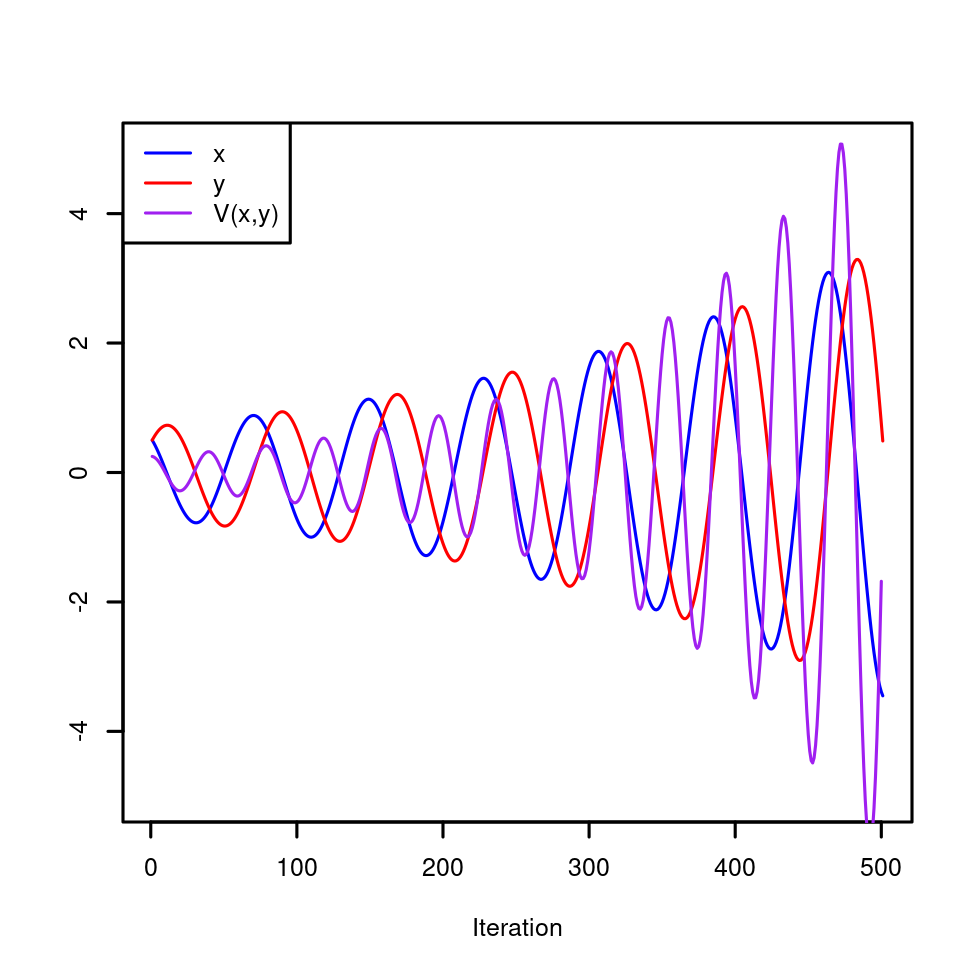
\includegraphics[width=0.6\textwidth]{plot1}
    \caption{Oscillating around the optimal value}
    \label{fig:alternating}
  \end{figure}
\end{example}

As we alternate updates, we observe oscillating behavior as depicted
in Figure \ref{fig:alternating}.  This oscillation has been observed
in GAN training.

% \begin{example}
%   We can do something similar with another value
%   function $V(x, y) = \log(x) + \log(1 - xy)$, with the same game
%   \begin{align}
%     \min_x\max_y V(x, y) = \log(x) + \log(1 - xy).
%   \end{align}
%   The updates for this optimization are
%   \begin{align}
%     x^{(t+1)} & \gets x^{(t)} - \eta \left( {1 \over x} + {y
%                 \over 1 - xy} \right); \\
%     y^{(t+1)} & \gets y^{(t)} - \eta \left({x \over 1 - xy} \right);
%   \end{align} and we can observe the following behavior in
%   Figure~\ref{fig:drop}.
%
%   \begin{figure}[H] \centering
%     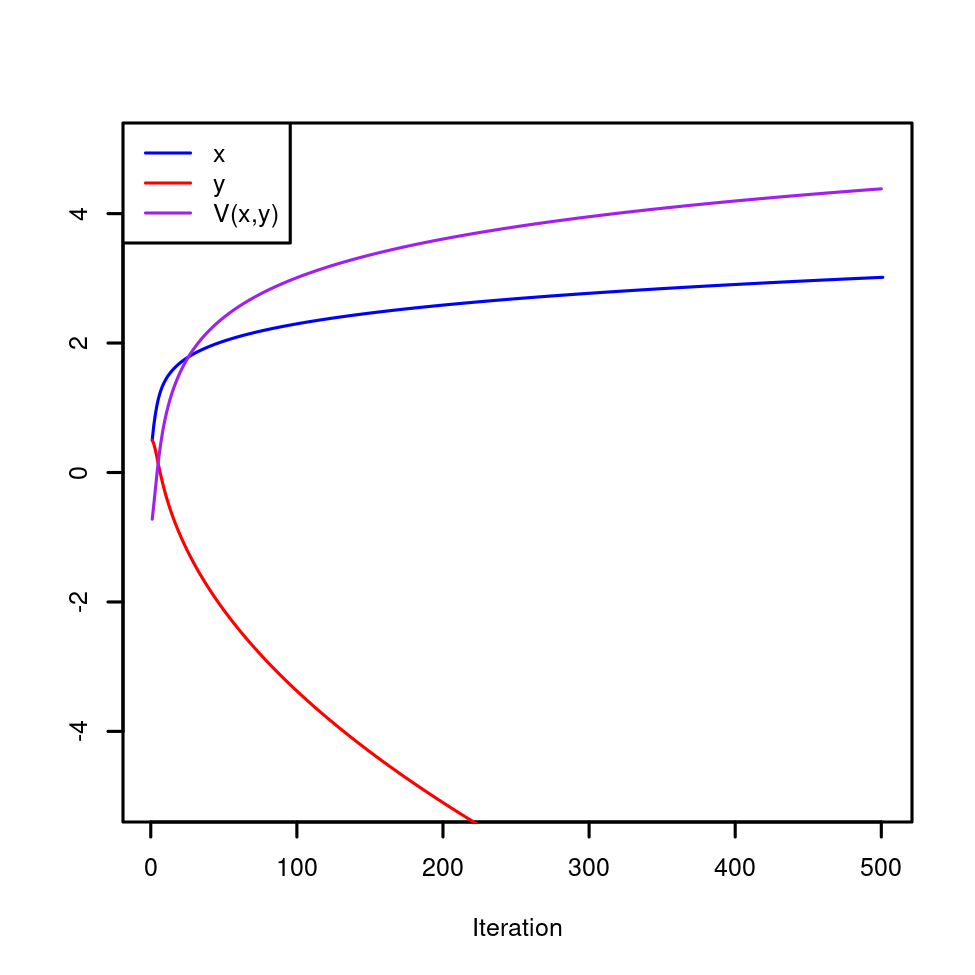
\includegraphics[width=0.6\textwidth]{plot2}
%     \caption{$x$ dominates}
%     \label{fig:drop}
%   \end{figure}
%
% \end{example}
%
% In the first example the optimization oscilates around 0, while in the
% second example $x$ quickly dominates, and this simple example
% resembles what happens in GAN training in practice.

\subsubsection{Two Value Functions}
\label{sec:two-value}

In \cite{ref:goodfellow-original}, the paper introduced one value
function as part of the theoretical discussion, but when it came to
training the algorithm, they used a different value function which
avoided the above issues. The first value function (equation
\ref{eq:the-original-objective-function}) is hard to train and often
leads to vanishing gradients, which means the generator has nothing to
learn from. The decoupled objective functions
\begin{align}
  \label{eq:second-value-function} \max_{\theta} \left(
  \mathbb{E}\left[\log{D_\theta(x)}\right] +
  \mathbb{E}\left[\log(1 - D_\theta(G_\phi(z)))\right]
  \right) \\
  \max_{\phi}\mathbb{E}\left[\log(D_\theta(G_\phi(z)))\right]
\end{align} have the same fixed points as the previous one, but the
gradients of the loss with respect to the generator are stronger,
therefore providing better learning material for the generator. With
equation \ref{eq:second-value-function} as the objective functions,
the GAN algorithm is no longer a zero-sum game.

\subsection{Generative Adversarial Networks}

The full algorithm is presented below.

\begin{figure}[H] \centering
  \begin{minipage}{0.95\linewidth}
    \begin{algorithm}[H]
      Let $\eta > 0$, \textit{be the learning rate.} \\
      Let $T > 0$, \textit{be the number of training iterations.} \\
      Let $\D: \Theta \times \&X \mapsto [0, 1]$ \\
      Let $\G: \Phi \times \&Z \mapsto \&X$ \\
      \While {t < T} { Let $z = \{z_1, \dots, z_m\}$, \textit{where
          each $z_i$ is sampled from $(\&Z, \pz)$
          This batch will be used in the optimization of $\D$.} \\
        Let $x = \{x_1, \dots, x_m\}$, \textit{where each $x_i$
          is from the training data.} \\
        Let
        $\theta \gets \theta + \eta \cdot \nabla_{\theta} {1 \over m}
        \sum_{i=1}^m \left[ \log{\D\left( x_i\right)} + \log{\left(1 -
              \D\left(\G\left( z_i\right)\right)\right)} \right]$,
        \textit{i.e.\ we update the discriminator's parameters
          $\theta$ by
          ascending the gradient of $\V$ with respect to $\theta$.} \\
        Let $z = \{z_1, \dots, z_m\}$, \textit{we sample a new batch
          from $(\&Z, \pz)$. This batch will be used in the
          optimization
          of $\G$.} \\

        $\phi \gets \phi - \eta \cdot \nabla_{\phi} {1 \over m}
        \sum_{i=1}^m \log{\left(1 -
            \D\left(\G\left(z_i\right)\right)\right)}$, \textit{i.e.\
          we update the generator's parameters $\phi$ by descending
          the gradient of $\V$ with respect to $\phi$.} \\ }
    \caption{Generative Adversarial Networks}
    \label{algo:main-algo}
  \end{algorithm}
  \end{minipage}
\end{figure}

In the original paper, the discriminator is said to be optimized $k$
times before the generator is optimized, however $k=1$, so we chose to
leave out that inner training loop in favor of readability conceptual
clarity.

\subsection{Discussion}

The minimax strategy for $D$ can be thought of as follows.  If $D$
assumes $G$ has done its worst, then $D$ should assume that $G$ is
able to produce data points that are indistinguishable from the real
thing. If that's the case, to minimize loss, $D$ should return
${1 \over 2}$ for all data points, which happens to be the maximum
entropy distribution over the two states (real or synthetic).  If
$D(x) = {1 \over 2}$ $\forall x$, there is nothing for $G$ can do to
improve its situation.  The next section will show
$D(x) = {1 \over 2}$ $\forall x$ is indeed the optimal strategy for
$D$.

%%% Local Variables:
%%% mode: latex
%%% TeX-master: "../thesis"
%%% End:
